\subsection{Anexo I}
\label{sec:anexo1}

La presente implementación se realizó utilizando una implementación
de \emph{Needleman-Wunsch} que proveen los módulos de python~\footnote{\url{http://pypi.python.org/pypi/nwalign/}}.

Se utilizó pues resultó ser mucho más óptima que una implementada por nosotros,
lo que se debe a que se la programación del módulo \emph{nwalign} utilizá programación
en \emph{cython}~\footnote{\url{http://www.cython.org/}}, lo que hace que el funcionamiento
sea más rápido por las extensiones utilizadas proveniente de módulos en \emph{C},
que tienen como objetivo principal, mejorar el rendimiento del código en python.


\lstset{
  literate={á}{{\'a}}1
           {é}{{\'e}}1
           {í}{{\'i}}1
           {ó}{{\'o}}1
           {ú}{{\'u}}1
}
\begin{small}
	\lstinputlisting{scripts/pregunta-2.py}
\end{small}

\newpage
\subsection{Anexo II}
\label{sec:anexo2}
\begin{small}
	\lstinputlisting{scripts/pregunta-3.py}
\end{small}

\newpage
\subsection{Anexo III}
\label{sec:anexo3}
\begin{small}
	\lstinputlisting{src/4.1-alineamiento.txt}
\end{small}

\newpage
\subsection{Anexo IV}
\label{sec:anexo4}
\begin{small}
	\lstinputlisting{src/4.2-alineamiento.txt}
\end{small}

\newpage
\subsection{Anexo V}
\label{sec:anexo5}
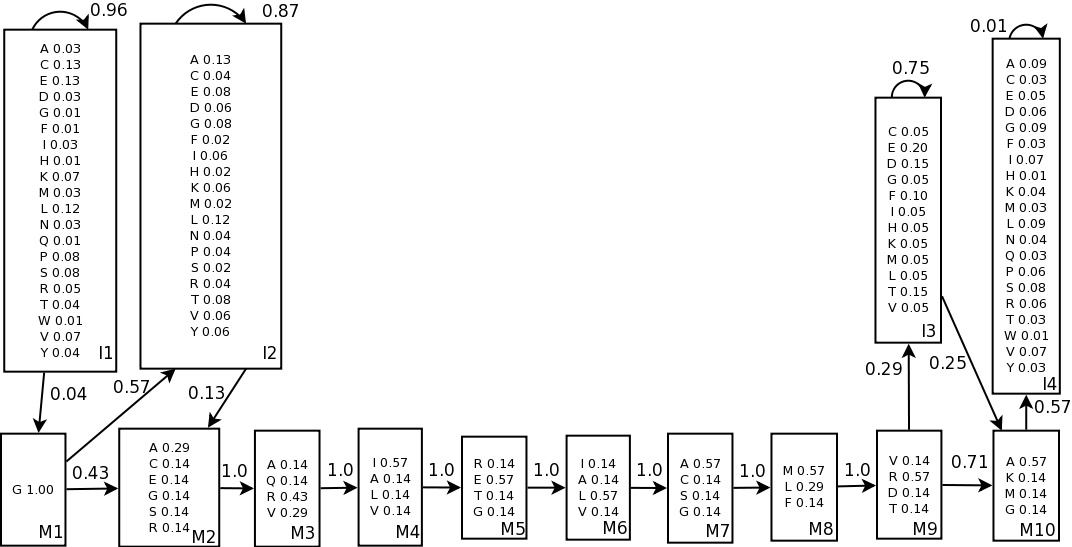
\includegraphics[angle=270,scale=0.55]{img/hmm}
